
В ходе проведения компьютерной экспертизы может потребоваться извлечение всех 
возможных контакт-листов злоумышленника, сохраненных локально различными 
программами, в особенности программами мгновенного обмена сообщениями. 


Программы мгновенного обмена сообщениями (Instant Messenger, IM) --- программы-клиенты, предназначенные   для обмена сообщениями в реальном времени через Интернет. С их помощью могут передаваться текстовые сообщения, звуковые сигналы, изображения, видео. Многие из таких программ-клиентов могут применяться для организации групповых текстовых чатов или видеоконференций.


Потребовалось проведение сравнительного анализа подобного рода программ-клиентов 
(ICQ, Pidgin, irc, Skype, Google Hangouts, Miranda IM и др.), 
в результате чего для разработки программного модуля в рамках проекта
<<Компьютерная экспертиза>> была выбрана программа ICQ. 


ICQ является централизованной службой мгновенного обмена сообщениями, использующей протокол OSCAR
и локализованно хранящей различного рода информацию о пользователе: переданные и полученные 
электронные сообщения и файлы,а также список контактов.


В результате исследования данной службы была получена информация о структуре хранения данных ICQ. Это, в свою очередь, позволило написать программный модуль, позволяющий извлекать 
контакт-лист из файлов, сохраняемых ICQ на жестком диске злоумышленника. 

\subsubsection{Общие сведения о программах мгновенного обмена сообщениями}

В ходе проведения сравнительного анализа программ-клиентов обмена мгновенными сообщениями
исследовались и сравнивались основные функции различных программ, их версии и год популярности.
Результаты данного исследования представлены в таблице~\ref{tab:messengers}.

% \newpage
% \ESKDthisStyle{empty}

\begin{center}
\begin{longtable}{|p{2cm}|p{2cm}|p{7cm}|p{5cm}|}
\caption{Результаты сравнительного анализа программ-клиентов обмена мгновенными 
сообщениями} %\endhead
\label{tab:messengers}

\hline
Имя & Год популярности & Основные функции & Текущая версия\\
\hline
ICQ & 
1990-ые & 
Микроблогинг, текстовые сообщения, заметки и напоминатели, аудио/видео сообщения, видеозвонки,
отправка файлов, изображений и видео, звонки на мобильные и городские телефоны, поддержка популярных социальных сетей; & 
8.2 Build 7135 (Windows) --- 2 сентября 2014 года
1.3.1 (Mac OS X) --- 10 июля 2014 года
Linux (beta) --- 22 апреля 2011 года \\
\hline
Pidgin & 2007 & Метаконтакты, запись протокола событий, поддержка вкладок в окне разговора,
подключение к нескольким аккаунтам одновременно, модульная структура, установка аватаров, настраиваемые сигналы действий пользователей, интеграция с GNOME, обмен файлами, кроссплатформенность; & 
2.10.9 (2 февраля 2014) \\
\hline
irc & 
1991 & 
Текстовые сообщения, групповое/приватное общение, обмен файлами; & 
1.2.5-alt1 
(2010-04-05) \\
\hline
Skype & 
2014 & 
Текстовые сообщения (чат), видеозвонки, конференц-звонки, обмен файлами, звонки на мобильные и стационарные телефоны, передача изображения с монитора; & 
Windows: 6.18.66.106 (5 августа 2014);
Windows 8.1: 2.8 (7 мая 2014);
Linux x86: 4.3.0.37 (18 июня 2014);
Mac OS X: 6.19 (9 июля 2014); \\
\hline
Google Hangouts & 
2013 - 2014 & 
Видеоконференции, текстовые сообщения, онлайн трансляция через Youtube, обмен файлами, групповой чат, звонки на  мобильные и стационарные телефоны; & 
Последняя версия --- 2.0 \\
\hline
Line &
2014 &
Текстовые сообщения, аудио- и видеозвонки, передача файлов; имеет встроенную социальную сеть, в которой поддерживаются блоги и комментарии; &
Последняя версия — 4.0.0 (03/09/2014) \\
\hline
Miranda IM &
2005 &
Текстовые сообщения, обмен SMS-сообщениями с мобильными устройствами, поддержка плагинов;
возможность определения приложения, при помощи которого работает собеседник;
в контакт-листе выдает полные сведения о контакте, включая внешний IP-адрес;
голосовая и видеосвязь отсутствуют; &
0.10.24 (9 сентября 2014) \\
\hline
Yahoo! Messenger &
2012 &
Текстовое сообщение, голосовое сообщение (в частности многопользовательский голосовой чат), видеоконференции, звонки на мобильные и стационарные телефоны, обмен файлами; &
11.5 (Windows) / 2.5.3 (Mac) / 1.0.6 (Unix) (15 января 2012 (Windows)) \\
\hline
Viber &
2013 - 2014 &
Бесплатные звонки через Wi-Fi и сети 3G, текстовые сообщения, передача изображений, видео- и аудиосообщения; &
Latest version:
4.1.0.1703 \\
\hline
Mail.Ru Агент &
2010 - 2011 &
Текстовые сообщения, IP-телефония, видеозвонки и отправка SMS,  микроблогинг, конференции, обмен файлами. &
Windows: 6.3, сборка 8050 — 2 сентября 2014;
OS X: 4.0.2 — 29 мая 2014; \\
\hline
MySpace IM &
2009 &
Поддержка Skype, 
звонки на сотовые телефоны с ПК, возможность получить собственный локальный номер с голосовой почтой
обмен тесктовыми сообщениями с другими пользователями MySpace;
настройка уровня прозрачности для списка контактов и окна чата;
журнал сообщений, а также его гибкая настройка;
настройка прокси-сервера. &
1.0.823.0 (1 декабря 2009 года) \\
\hline
QIP IM  &
2010 &
Поддержка внешних плагинов, уведомления о новой почте, обмен файлами и текстовыми сообщениями (в т.ч. SMS), аудио- и видеозвонки,
интеграция с популярными соцсетями. &
QIP 2012 — версии 4.0 (сборка 9379) (23 июня 2014 года); \\
\hline
Zoho Chat &
2010 &
Групповой вэб - чат, интеграция с Yahoo, AIM, MSN, ICQ, GTalk и Jabber, обмен сообщениями с незарегистрированными в Zoho пользователями через браузер. &
05.08.10 Zoho Chat \\
\hline
\end{longtable}
\end{center}


На выбор  программы-клиента для реализации программного модуля повлияло не только исследование программ мгновенного обмена сообщениями, но и уровень развития навыков разработчика, а также были исключены программы Pigin и Skype, поскольку данные модули были разработаны ранее. 


Далее потребовалось ознакомиться с самим приложением ICQ версии 8.2, найти директорию, в которой хранится необходимая информация, изучить форматы и содержимое найденных файлов. 


Для идентификации пользователей служба ICQ использует UIN (Universal Identification Number) --- уникальный для каждой учётной записи номер, состоящий из 5-9 арабских цифр. Этот номер присваивается учётной записи при первичной регистрации пользователя в системе, после чего, в паре с паролем, может использоваться для аутентификации в системе. Контакты злоумышленника будут храниться в виде пар 
значений --- <<ника>> (nick) пользователя и его идентификационного номера (email) --- разделе C:\textbackslash Users\textbackslash UserName\textbackslash AppData\textbackslash Roaming\textbackslash ICQ - Profile. 


Данная информация сохраняется программой ICQ в XML - документе, пример которого представлен на рисунке~\ref{xml_view:xml_view}). Каждый xml-тэг соответствует одному элементу контактного листа и содержит значения атрибутов <<nick>> и <<email>>, которые и будут считываться программой и сохраняться в выходной файл.

\begin{figure}[h!]
\center{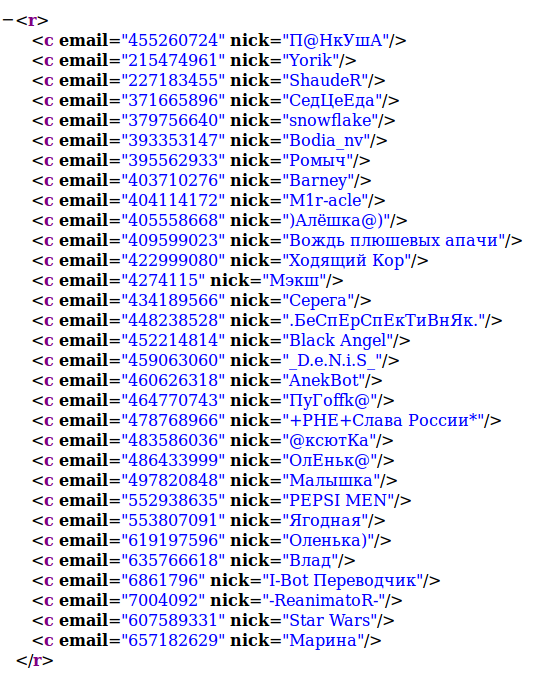
\includegraphics[width=0.6\linewidth]{xml_view}}
\caption{Список контактов пользователя в формате XML}
\label{xml_view:xml_view}
\end{figure}


\subsubsection{Реализация программного модуля}

Реализация программного модуля включала в себя следующие шаги:

\begin{enumerate}
\item Изучение проекта coex;
\item Изучение особенностей работы с библиотеками QT;
\item Изучение особенностей работы с XML-форматом (языка разметки);
\item Изучение системы компьютерной верстки  Latex для написания документации;
\item Изучение системы распределенного контроля версий Git и ее основных возможностей; 
\item Установка ICQ 8.2 на виртуальную машину с операционной системой Windows 7;
\item Создание информационной базы для исследования (нескольких аккаунтов, обмен соощениями и файлами);
\item Разработка программного модуля.
\end{enumerate}


\subsubsection{Алгоритм работы модуля}
Алгоритм работы модуля выглядит следующим образом: на вход программе подается XML-документ, в котором приложение ICQ хранит контактный лист пользователя. Выполняется проверка, является ли данный файл доступным для чтения. Если он таковым является, то далее создается потоковая переменная, в которую считывается информация из файла, а затем программа находит значения нужных нам атрибутов <<email>> и <<nick>>, записывая найденные значения в выходной файл, который также будет иметь формат XML-документа. Операция будет выполняться до тех пор, пока не будет достигнут конец файла, после чего файл благополучно закрывается и завершается выполнение программы.


Алгоритм синтаксического анализа входного XML--файла, содержащего контакт-лист, представлен на блок--схеме ниже (рис.~\ref{block_diagram:block_diagram}).

\begin{figure}[h!]
\center{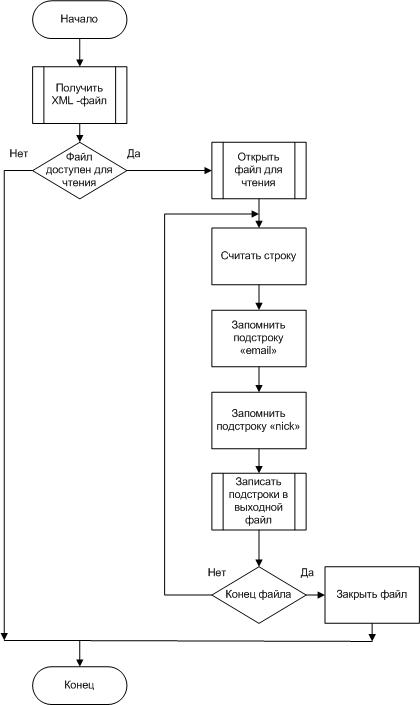
\includegraphics[width=0.6\linewidth]{block_diagram}}
\caption{Блок-схема синтаксического анализа входного файла}
\label{block_diagram:block_diagram}
\end{figure}

Исходный код функции синтаксического анализа контактного листа приложения ICQ можно увидеть на рисунке~\ref{my_code:my_code}.

\begin{figure}[h!]
\center{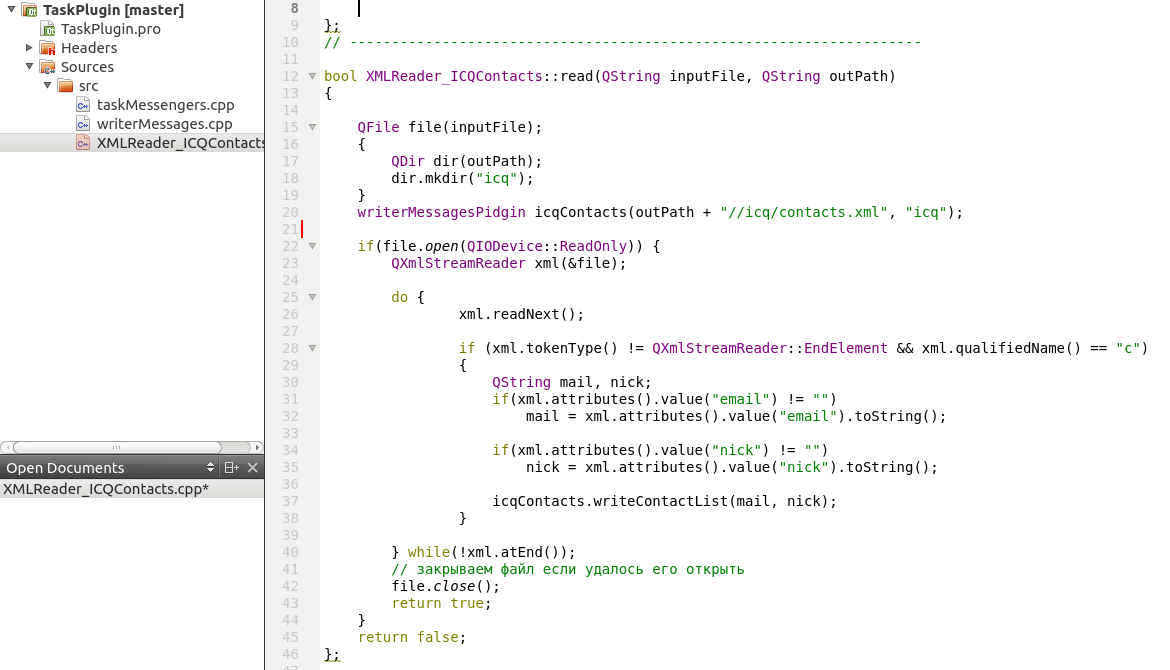
\includegraphics[width=0.9\linewidth]{my_code}}
\caption{Исходный код функции синтаксического анализа контактного листа приложения ICQ}
\label{my_code:my_code}
\end{figure}

Пример результата работы модуля в виде файла в формате XML представлен на рисунке~\ref{output_xml:output_xml}.

\begin{figure}[ht]
\center{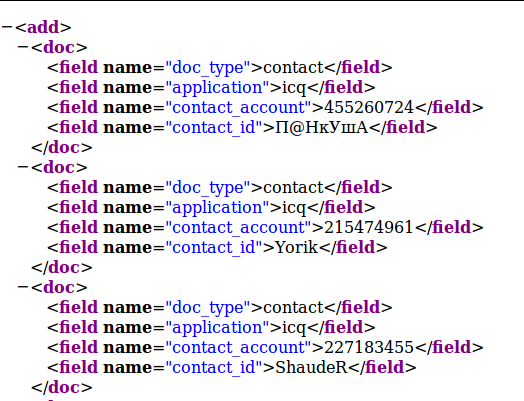
\includegraphics[width=0.6\linewidth]{output_xml}}
\caption{Пример результата работы модуля в виде файла в формате XML}
\label{output_xml:output_xml}
\end{figure}

\subsubsection{Здачи на следующий семестр}

В дальнейшем планируется дополнить модуль функцией рекурсивного обхода файловой системы для нахождения необходимых файлов, а также функциями для синтаксического анализа файлов с сообщениями злоумышленника.

\clearpage
